\documentclass[11pt]{article}
\usepackage{classTools}

\begin{document}
% To include a problem set header, use the psHeader command
\psHeader{2}{Wed 2024-09-25 (11:59pm)}

\textbf{Your name: } Emily Kang

\textbf{Collaborators: } Vennela Jonnala

\textbf{No. of late days used on previous psets: } 0

\textbf{No. of late days used after including this pset: } 0
\\

Please review the Syllabus for information on the collaboration 
policy, grading scale, revisions, and late days.

\begin{enumerate}
     \item  (designing reductions) 
     The purpose of this exercise is to give you practice designing reductions and proving their correctness and runtime.
    Consider the following computational problem:

    \compprob{AreaOfConvexPolygon()}
    {Points $(x_0,y_0),\ldots,(x_{n-1},y_{n-1})$ in the $\R^2$ plane that are the vertices of a convex polygon (in an arbitrary order) whose interior contains the origin}
    {The area of the polygon formed by the points}


    \begin{enumerate}
        \item \label{part:polar} 
        Show that AreaOfConvexPolygon$\leq_{O(n),n}$ Sorting.  Be sure to analyze both the correctness and runtime of your reduction.

        In this part and the next one, you may assume that a point $(x,y)\in \R^2$ can be converted into polar coordinates $(r,\theta)$ in constant time. 
        \\\\
        You may find the following useful (and you may use them without proof):
        \begin{itemize}
            \item The polar coordinates $(r,\theta)$ of a point $(x,y)$ are the unique real numbers $r\geq 0$ and $\theta\in [0,2\pi)$ such that $x=r\cos \theta$ and $y=r\sin \theta$. Or, more geometrically, $r=\sqrt{x^2+y^2}$ is the distance of the point from the origin, and $\theta$ is the angle between the positive $x$-axis and the ray from the origin to the point.
            \item The area of a triangle is $A = \sqrt{s(s-a)(s-b)(s-c)}$ where $a, b, c$ are the side lengths of the triangle and $s = \frac{a + b + c}{2}$ (\href{https://en.wikipedia.org/wiki/Heron\%27s_formula}{Heron's Formula}).
        \end{itemize}
        \textit{Solution.} 
        \begin{enumerate}
            \item \textbf{Runtime Analysis:} The problem is dominated by the sorting of the array of polar coordinates. Using \texttt{MergeSort}, the runtime of the sorting takes $O(n\log n)$ time. The preprocessing, or reduction, takes $O(n)$. The postprocessing also takes $O(n)$ time. (See 1(b) for more details.)
            \item \textbf{Proof of Correctness:} First, we will analyze the correctness of \texttt{AreaofConvexPolygon}. The function \texttt{AreaofConvexPolygon} will indeed take an input of $n$ points in arbitrary order whose interior contains the origin and will output the area of the polygon formed by the points.

            Using the hint, we know that we can represent each of the $n$ points in polar form. Then, we can sort the points in polar form using a reduction to sorting, which can sort the $n$ polar coordinates in increasing order of $\theta$. From the sorted list of polar coordinates, we make pairs of adjacent coordinates $[((\theta_0, r_0), (\theta_1, r_1)), \dots, ((\theta_{n-1}, r_{n-1}), (\theta_0, r_0))]$ (note how the indices wrap around back to $0$ at the end). 

            We can then form $n$ triangles where the vertices of each triangle are a pair of points and the origin. We know that these triangles are disjoint and partition the polygon. Therefore, if we find the individual areas of each of the $n$ triangles and take their sum, the sum will be equal to the area of the polygon.

            To find the area of each individual triangle, we can use the distance formula to find the side lengths of the triangle, and then use Heron's Formula (as per the hint) to calculate the area. After we have calculated all the areas of the disjoint triangles that partition the polygon, we can take their sum. This will give us the area of the polygon formed by the points given in the input.
        \end{enumerate}

        \item Deduce that AreaOfConvexPolygon can be solved in time $O(n\log n)$. \\
        \textit{Solution.} Let \texttt{MergeSort} be the algorithm that sorts the array of $n$ polar coordinates in increasing order of $\theta$. The time complexity of \texttt{MergeSort} is $O(n\log n)$ for an array of length $n$.

        First, we preprocess the input by converting each of the $n$ points to polar coordinates. Since converting a point to polar coordinates takes constant time, the total preprocessing time is $O(n)$.

        Next, \texttt{MergeSort} is applied to the array of $n$ polar coordinates, which takes $O(n \log n)$ time. 

        After sorting, we traverse the sorted list and create $n$ pairs of adjacent polar points. For each pair, we perform mathematical operations to compute the area of the triangle formed by the pair and the origin. These operations are done in constant time for each pair, resulting in $O(n)$ time for this step.

        Finally, we sum the areas of the $n$ triangles, which takes $O(n)$ time.

        Therefore, the overall time complexity is $O(n)$ for preprocessing, $O(n\log n)$ for sorting, $O(n)$ for creating pairs and calculating areas, and $O(n)$ for summing the areas. Thus, the total runtime is 
        \[
        O(n) + O(n\log n) + O(n) + O(n) = O(n\log n).
        \]
        
        \item (*challenge; extra credit; optional\footnote{This problem is meant to be done based on your enjoyment/interest and only if you have time. It won't make a difference between N, L, R-, and R grades (meaning it will only impact whether an R gets increased to an R+), and course staff will deprioritize questions about this problem at office hours and on Ed.})  Come up with a way to avoid conversion to polar coordinates and any other trigonometric functions in solving AreaOfConvexPolygon in time $O(n\log n)$.  Specifically, design an $O(n)$-time reduction that makes $O(1)$ calls to a Sorting oracle on arrays of length at most $n$, using only arithmetic operations $+$, $-$, $\times$, $\div$, and $\sqrt{\hspace{1em}}$, along with comparators like $<$ and $==$.  (Hint: first partition the input points according to which quadrant they belong in, and consider the slope of the line from a vertex (x,y) to the origin.) \label{part:nopolar} \\
        \textit{Solution.} Let us design a solution to the \texttt{AreaOfConvexPolygon} problem without converting points to polar coordinates or using trigonometric functions. 

        \begin{enumerate}
            \item \textbf{Quadrant Partitioning:} First, we partition the points based on the quadrant they fall into. We can create 4 dictionaries, one for each quadrant. The points $(+, +)$ belong to the first quadrant, $(-, +)$ to the second, $(-, -)$ to the third, and $(+, -)$ to the fourth. This partitioning step can be done in $O(n)$ time as we simply traverse the input array once.
            
            \item \textbf{Calculate Slopes:} For each point in the quadrants, we calculate the slope of the line passing through the origin and the point using the formula $slope = \frac{y}{x}$. We store the points in the dictionary with the slope as the key and the point as the value. Calculating the slope for each point is a constant-time operation, and since we are processing all $n$ points, this step also takes $O(n)$ time.
            
            \item \textbf{Sort by Slope:} Next, for each quadrant, we sort the points based on their slopes. We apply \texttt{MergeSort} to each of the 4 dictionaries (one per quadrant). Sorting each dictionary of size $n/4$ takes $O\left(\frac{n}{4} \log \frac{n}{4}\right)$ which simplifies to $O(n \log n)$ in total for all 4 dictionaries. This ensures that the points within each quadrant are sorted by their increasing slope values.
            
            \item \textbf{Combine Quadrants:} Once the points are sorted by slope within each quadrant, we concatenate the points from all four quadrants into a single list, preserving the order of the quadrants: first quadrant, second quadrant, third quadrant, and finally the fourth quadrant. This step takes $O(n)$ time.
            
            \item \textbf{Compute Areas:} Now, with the points ordered, we can proceed to calculate the area of the polygon. We pair adjacent points and compute the area of the triangles formed by each pair of points and the origin. This is done using only arithmetic operations (addition, subtraction, multiplication, and division). This process is the same of that from question 1(a)(ii), the proof of correctness. Again, this method works since the triangles form disjoint sections that partition the polygon. The total time for this step is $O(n)$.
            
        \end{enumerate}

        The total runtime includes of $O(n)$ time for partitioning, calculating slopes, combining quadrants, and computing areas, and $O(n \log n)$ for sorting the points by slope within each quadrant. Thus, the final time complexity is:
        $
        O(n) + O(n \log n) = O(n \log n).
        $
    \end{enumerate}
    
    Similar techniques to what you are using in this problem are used in algorithms for other important geometric problems, like finding the Convex Hull of a set of points, which has applications in graphics and machine learning.

    \item (composition of reductions) 
    The purpose of this exercise is to give you practice in working with the abstract definition of reductions.
    
    Let $\Pi, \Gamma, \Lambda$ be computational problems, and suppose that $\Pi\leq_{T_1(n),q_1(n)\times h_1(n)} \Gamma$ and $\Gamma \leq_{T_2(n),q_2(n)\times h_2(n)} \Lambda$, for non-decreasing functions $T_1,T_2,q_1,q_2,h_1,h_2$.  Determine functions $T_3,q_3,h_3$ in terms of $T_1,T_2,q_1,q_2,h_1,h_2$ such that 
    $$\Pi \leq_{O(T_3(n)),q_3(n)\times h_3(n)} \Lambda,$$
    and justify your answers. 
    (Hint: you can take $h_3(n)=h_2(h_1(n))$.) \\
    \textit{Solution.} 
    \begin{enumerate}
        \item $T_3(n) = T_1(n) + q_1(n)\cdot T_2(h_1(n)).$ Preprocessing and postprocessing take $T(n)$ for $\Pi,$ and for each of the $q_1(n)$ times $\Gamma$ runs, it must also have its own preprocessing and postprocessing, which each time take $T_2(h_1(n))$ since the input to $\Gamma$ is of size $h_1(n).$
        \item $q_3(n) = q_1(n)\cdot q_2(h_1(n)).$ For each of the $q_1(n)$ calls within $\Pi,$ there are $q_2(h_1(n))$ calls within $\Gamma,$ keeping in mind the current input size of $h_1(n).$
        \item $h_3(n) = h_2(h_1(n)).$ $\Lambda$ takes in $h_2$ of the previous input, which is $h_1$ of the original input, $n.$
    \end{enumerate}

    
    \item (augmented binary search trees) The purpose of this problem is to give you experience reasoning about correctness and efficiency of dynamic data-structure operations, on variants of binary-search trees. 
    
    Specifically, we will work with {\em selection data structures}.
    We have seen how binary search trees can support min queries in time $O(h)$, where $h$ is the height of the tree.  A generalization is {\em selection} queries, where given a natural number $q$, we want to return the $q$'th smallest element of the set.  So $\texttt{DS.select(0)}$ should return the key-value pair with the minimum key among those stored by the data structure $\texttt{DS}$, $\texttt{DS.select(1)}$ should return the one with the second-smallest key, $\texttt{DS.select(n-1)}$ should return the one with the maximum key if the set is of size $n$, and $\texttt{DS.select((n-1)/2)}$ should return the median element if $n$ is odd.
    
    In the Roughgarden text (\S11.3.9), it is shown that if we {\em augment} binary search trees by adding to each node $v$ the size of the subtree rooted at $v$, then Selection queries can be answered in time $O(h)$.\footnote{Note that the Roughgarden text uses a different indexing than us for the inputs to Select. For Roughgarden, the minimum key is selected by Select(1), whereas for us it is selected by Select(0).}
    
    \begin{enumerate}
        \item In the Github repository, we have given you a Python implementation of size-augmented BSTs supporting search, insertion, and selection, and with a stub for \texttt{rotate}. One of the implemented functions (\texttt{search}, \texttt{insert}, or \texttt{select}) has a correctness error, another one is too slow (running in time that's (at least) linear in the number of nodes of the tree rather than linear in the height of tree), and the third is correct.
        
        Identify and correct these errors. You should provide a text explanation of the errors and your corrections, as well as implement the corrections in Python. \\
        
        \textit{Solution.}
            \begin{enumerate}
                \item \texttt{search}: The implementation is correct.
                \item \texttt{insert}: The runtime is too slow. This is because at the end of the implementation, \texttt{calculate\_sizes} is called on the entire tree, recalculating the sizes for the entire tree with runtime $O(n)$ as we traverse every node to calculate the size. However, we can update the sizes as we go, adding $1$ to only each node we traverse on our way to insert the input \texttt{key}. This is better in terms of runtime because incrementing a size by $1$ takes constant time for nodes in the tree that we are already visiting within the function, which means this would not impact our worse-case runtime.
                \item \texttt{select}: There is a correctness error in this function implementation. When we haven't yet found the index and we traverse the left subtree, it makes sense to call \texttt{select} again with the left subtree and the index, since this index is referencing the minimum key, and the left tree's minimum is the minimum of the entire tree, so everything stays relative. However, when we haven't found the index yet and we traverse the right subtree, we've readjusted our new relative minimum to be the minimum of the right subtree. This can be larger than the minimum of the entire tree, therefore we have to account for the "new" minimum. We can do that by simply replacing the original index with \texttt{$ind - left_size - 1$} as this accounts for us disregarding the entire left subtree and adjusting to only considering the right subtree.
    
            \end{enumerate}

        \item Describe (in pseudocode or pictures) how to extend \texttt{rotate} to size-augmented BSTs, and argue that your extension maintains the runtime $O(1)$. Prove that your new rotation operation preserves the invariant of correct size-augmentations. (That is, if every node's size attribute had the correct subtree size before the operation, then the same is true after the operation.)
        
        \textit{Solution.} To extend \texttt{rotate} to size-augmented BSTs, we must carefully identify when we need to recalculate the size of a subtree. Below is a possible pseudocode.
        \begin{figure}[H]
            \centering
            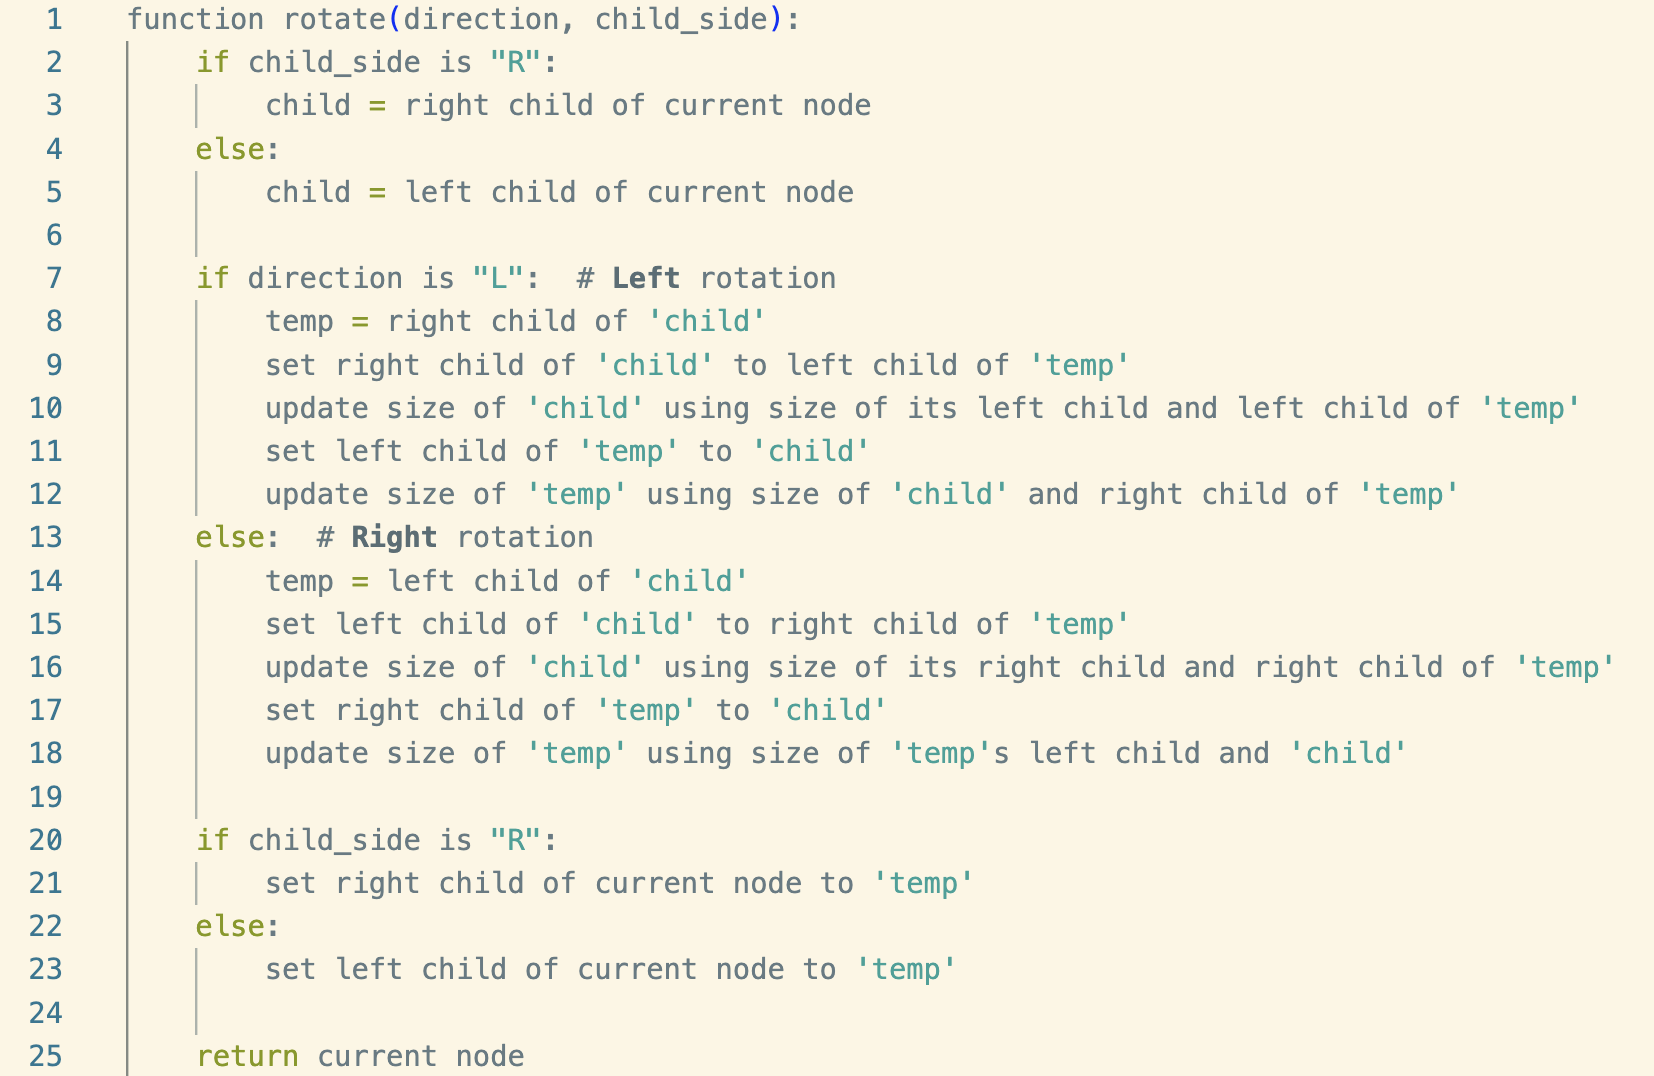
\includegraphics[width=\linewidth]{pseudocode.png}  % Width can be adjusted as needed
            \caption{Pseudocode for the extended \texttt{rotate} function}
            \label{fig:pseudocode}
        \end{figure}
        This extension would maintain the runtime $O(1).$ In the original \texttt{rotate}, the runtime was $O(1)$ because we were simply rearranging the pointers between a fixed number of nodes (the child and a few of its children). This would take constant time regardless of the size of the entire tree. When we extend \texttt{rotate} we need to update the sizes of the nodes that we traversed. To update, we do simple math operations of adding sizes which takes constant time. Again, since this is for a constant number of nodes no matter the size of the tree, we maintain the constant runtime of $O(1)$. \\

        The new rotation operation also preserves the invariant of the correct size-aumentation. Assume that every node's size attribute had the correct subtree size before the operation. After a rotation, only the size of the node being rotated and its child change. Therefore we only need to make sure that the size of these two nodes are correct after the rotation, where size is calculated as 
        $$
        1 + \text{size of left child} + \text{size of right child}
        $$
        For either a left rotation or a right rotation, the size of the grandchildren of the node being rotated do not change.
        \begin{enumerate}
            \item Left rotation: When a left rotation occurs, the size of the node being rotated and its right child are affected and therefore need to be updated. After the rotation is completed, the right child of the node being rotated takes its place, becoming the new parent, and the original node that was rotated becomes the left child. We update the new "parent" (originally the right child of the node being rotated) and the new "left child" (originally the node being rotated) as follows. Let us abreviate the new left child as $c$ and the new parent as $n$.
            $$
            \text{size of c} = 1 + \text{size of c's left child} + \text{size of c's right child}
            $$
            $$
            \text{size of n} = 1 + \text{size of c} + \text{size of n's right child}
            $$
            By assumption, we know that size of c's left and right child are correct, therefore the size of $c$ is correct. By assumption, we also know that the size of $n_p$'s right child is correct, therefore the size of $n_p$ is correct.
            \item Right rotation: When a right rotation occurs, the size of the node being rotated and its left child are affected and therefore need to be updated. The same reasoning applies as in the left rotation case. This time we abreviate the new \emph{right} child as $c$ and the new parent as $n$, as before.
            $$
            \text{size of c} = 1 + \text{size of c's left child} + \text{size of c's right child}
            $$
            $$
            \text{size of n} = 1 + \text{size of n's left child} + \text{size of c}
            $$
            By analogous assumptions as in the left case, we know that the size of $c$ and the size of $n_p$ are correct.
        \end{enumerate}
        Therefore we have shown that the new rotation operation preservers the invariant of correct size-augmentations.
        \item Implement \texttt{rotate} in size-augmented BSTs in Python in the stub we have given you.
    
    \end{enumerate}
    
    \emph{Food for thought (do read - it's an important take-away from this problem):} This problem concerns size-augmented binary search trees. In lecture, we discussed AVL trees, which are balanced binary search trees where every vertex contains an additional \textit{height} attribute containing the length of the longest path from the vertex to a leaf (height-augmented). Additionally, every pair of siblings in the tree have heights differing by at most 1, so the tree is height-balanced. Note that if we augment a binary search tree both by size (as in the above problem) and by height (and use it to maintain the AVL property), then we create a dynamic data structure able to perform \texttt{search}, \texttt{insert}, and \texttt{select} all in time $O(\log n)$. 


\item (reflection) We aim for cs1200 to be a collaborative learning community. Describe two concrete ways in which you have supported, or will try to support, your classmates' learning in the course.  Be specific, connecting your answer to the structure of cs1200. 

\textit{Note: As with the previous psets, you may include your answer in your PDF submission, but the answer should ultimately go into a separate Gradescope submission form.}

\item Once you're done with this problem set, please fill out \href{https://forms.gle/pyhGJ73HpodhThNP9}{this survey} so that we can gather students' thoughts on the problem set, and the class in general. It's not required, but we really appreciate all responses!

\end{enumerate}



\end{document}
